\documentclass[sigplan,screen,nonacm]{acmart}
\settopmatter{printfolios=true}

\usepackage{tikz}
\usetikzlibrary{arrows.meta,positioning,fit}
\usepackage{booktabs}
\usepackage{xspace}

\newcommand{\rvwmo}{RVWMO\xspace}
\newcommand{\vtwo}{machine~v2\xspace}
\newcommand{\code}[1]{\texttt{#1}}
\newcommand{\guard}[1]{\llbracket #1 \rrbracket}

\begin{document}

\title{Verifying RISC-V Programs on a Promising Machine}
\subtitle{A program logic, a faithful machine, and the road to xv6}

\author{Technical report}
\affiliation{\institution{xv6iris project}\country{}}
\date{5 November 2026}

\begin{abstract}
We describe a verification stack for concurrent RISC-V programs under the RISC-V weak memory model (\rvwmo),
mechanised in Lean~4 on iris-lean. Its core is an operational \emph{promising machine} in the style of
Promising-ARM/RISC-V~\cite{pulte19}, made faithful to the RISC-V manual by a systematic two-sided audit and driven by
the official Sail model. On top of it we build an Iris-style program logic whose per-hart weakest precondition
steps in program order yet handles load buffering, because it is parameterised by the run's final memory.
We prove its adequacy, a completeness theorem showing that every execution the manual's axiomatic model allows is a
run of the machine, and a prefix lemma covering infinite executions. Together they turn proofs in the logic into
theorems about the reference model itself: 25 forbidden litmus outcomes, including LB with data dependencies and
with fake dependencies, are so derived. We compare two ways of adding ownership transfer---a promises-first,
frontier-gated discipline (track~(a)) and lock-scoped pull promises over a release-in-place normal form
(track~(b))---evaluate them on spinlocks including xv6's exact \code{acquire}/\code{release} code, and select
track~(a). We close with what remains to verify the xv6 kernel on this foundation.
\end{abstract}

\maketitle

\section{Problem}

\rvwmo permits behaviours no in-order machine produces. The canonical one is load buffering (LB):
\begin{center}\small
\begin{tabular}{l||l}
hart 0 & hart 1\\\midrule
\code{r1 = ld x; sd y,1} & \code{r2 = ld y; sd x,1}
\end{tabular}
\end{center}
\noindent with outcome $r_1=r_2=1$ allowed: each load reads a store its author has not executed yet in program order.
Our previous attempt verified the xv6 kernel on an operational machine (MachCSL) that cannot produce LB, and then tried
to \emph{bridge} to \rvwmo by realising every axiomatic execution as a machine run. The bridge required a
program-specific ``cycle kill'' (no racy po\,$\cup$\,rf cycles in xv6), accumulated about ten unproved inputs, and at
three instructions realised a load with a value different from the hardware's. We abandoned it. The design goals of
the work reported here are:
(G1)~the logic must be sound \emph{directly} for an \rvwmo-faithful machine, with no program-specific transfer;
(G2)~the definition of \rvwmo is the RISC-V manual;
(G3)~the logic must stay compatible with the existing xv6 proof text.

\section{The Machine}

\paragraph{Taken from Promising-ARM/RISC-V.}
\vtwo follows Pulte et al.~\cite{pulte19}. Memory is one append-only list of messages; a message's timestamp is its
position; a \emph{view} is a timestamp. Each hart keeps registers paired with views, per-location coherence, the views
$v_{rOld}, v_{wOld}, v_{rNew}, v_{wNew}, v_{CAP}, v_{Rel}$, a forwarding bank, an exclusive bank and a set of promises.
Dependencies are syntactic: a register's view is the join of its sources', a branch raises $v_{CAP}$.
A hart may \emph{promise} a write at any time, appending it without running code; the store later \emph{fulfils} it,
which is allowed only when its pre-view (address, data, control dependencies, fences, release) is strictly below the
promised timestamp. Following Pulte's Theorem~6.2 we drop certification: a run is \emph{valid} when every promise is
fulfilled at the end.

\paragraph{What we changed.}
The paper's machine and its equivalence proof cover a small idealised ISA. We extended the machine, each change marked
\textsc{faithful}, \textsc{weaker} or \textsc{stronger} against quoted manual text: AMOs as single memory operations
with \code{.aq}/\code{.rl}; LR/SC with the manual's pairing rules, including mismatched pairs and failures; Zalasr
load-acquire/store-release as RCsc; instruction fetch with a per-hart floor raised by \code{fence.i}; every behaviour
the manual permits for misaligned accesses, \code{cbo.zero}, \code{cbo.inval} and failed \code{amocas}; byte-granular
messages with a single read point for mixed-size loads; nondeterministic answers for unmodelled hooks; and global
havoc after a Sail internal error. The machine consumes labels emitted by the official Sail RV64 model, with
translation off in this phase.

\paragraph{The fidelity audit.}
Before any proof we compared the machine against the manual in both directions: a code-side table extracted
mechanically from the Lean declarations (822 rows; a missing row fails the build), a spec-side table of every
normative sentence in scope, a kernel-checked decoder check over 1{,}041 encoding classes, and generated probe
families (e.g.\ 55{,}298 event-pair probes) compared on \emph{full outcome sets} against the reference. A calibration
run on our previous machine rediscovered every seeded defect, measuring the method's recall. The audit found and fixed
six machine defects (forwarding views of acquires, mismatched LR/SC, lost annotations, CSR read views, invalidate
views, and SC failure), and four bugs in external artefacts: herd treats Zalasr annotations as RCpc and forces
mismatched SCs to fail; the manual's own herd model has a typo and two omissions.

\section{Reference Model and Completeness}

\paragraph{The reference.}
\code{rvwmoRef} encodes the manual's axiomatic model at byte level: the 13 preserved-program-order rules, the load
value, atomicity and progress axioms, and the LR/SC success conditions. A reflective checker, proved sound and
complete, decides litmus verdicts by \code{decide}; 77 verdict theorems hold. On the litmus-tests-riscv corpus the
reference agrees with herd running the manual's own formal model on 7{,}863 tests; the three disagreements are
omissions of that formal model, where the reference follows the prose.

\paragraph{Completeness.}
\code{rvwmo\_complete} proves that every execution of the reference is a valid run of \vtwo with the same per-hart
observations, registers and final memory, for single-size programs with plain accesses, fences, AMOs, LR/SC and
acquire/release. Following Pulte's \code{AtoP}, the run promises all writes in global-memory order first and replays
each hart in program order; one step lemma per instruction class discharges the machine's premises from the \rvwmo
axioms. Acyclicity of the global memory order is used here once, program-agnostically; no proof assumes that a
program lacks cycles.

\paragraph{Infinite executions.}
\code{rvwmo\_prefix} shows that any finite set of observations of an infinite reference execution (with the progress
axiom read literally) is reproduced by a finite legal partial execution; the cut is everything up to the observations
in program order plus their global-memory-order predecessors, finite by progress. Composed with completeness, kernels
that never terminate are covered (currently for plain accesses and fences).

\section{The Logic and its Adequacy}

\paragraph{Weakest precondition.}
\code{wpPF} is an iris-lean weakest precondition for one hart, stepping through the machine's labels in program order,
one later and one credit per step. Its novelty is that it is \emph{parameterised by the run's final memory $M$}, a
prophecy: a load may return any message of $M$ its views allow, including one its author has not fulfilled yet. What
the hart learns from that value is \emph{guarded}: $\guard{V}\,\phi$ holds once every message up to $V$ is known to
satisfy the protocol. Register points-to carry views (\code{r $\mapsto_r$ v @ V}), and a trace invariant $\Psi$
records what each hart has observed. This answers the question that defeated graph-machine designs: a load reading a
not-yet-stepped store needs no backward step, because the store is already in $M$.

\paragraph{Adequacy (A0).}
\code{PF.adequacy} states: if every hart's \code{wpPF} holds, then for every valid run, $\Psi$ holds of every prefix of
every hart's trace, every message satisfies the protocol, finished harts' values satisfy their postconditions, and the
trace is well-formed against $M$. Figure~\ref{fig:chain} shows the proof. Given any valid run $R$---an arbitrary fixed
interleaving---a trace-preserving promises-first factorisation (Pulte's Theorem~7.1, proved here) yields each hart's
solo run against $M$. For the ownership logics a program-agnostic schedule lemma re-interleaves these into an
execution $R'$ of the proof language; Iris adequacy applies to $R'$, and its conclusions, which mention only $M$ and
per-hart traces, transfer to $R$. An independent review confirmed that the rescheduling preserves every load value
and read-from source.

\begin{figure}[t]
\centering
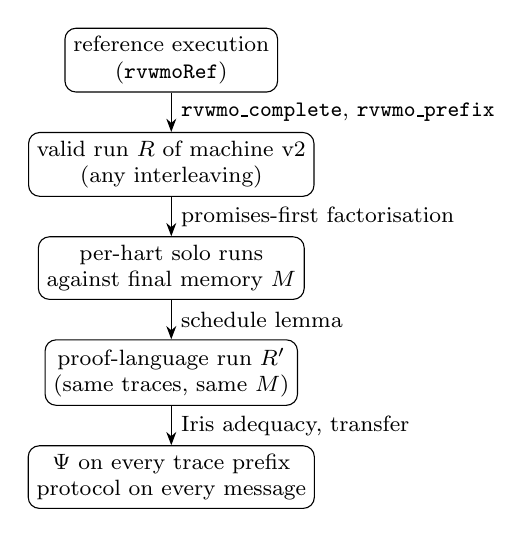
\begin{tikzpicture}[node distance=5mm, every node/.style={font=\footnotesize, align=center},
  box/.style={draw, rounded corners, inner sep=3pt, minimum width=24mm}, >={Stealth}]
\node[box] (ref) {reference execution\\(\code{rvwmoRef})};
\node[box, below=of ref] (run) {valid run $R$ of \vtwo\\(any interleaving)};
\node[box, below=of run] (solo) {per-hart solo runs\\against final memory $M$};
\node[box, below=of solo] (rp) {proof-language run $R'$\\(same traces, same $M$)};
\node[box, below=of rp] (facts) {$\Psi$ on every trace prefix\\protocol on every message};
\draw[->] (ref) -- node[right]{\code{rvwmo\_complete}, \code{rvwmo\_prefix}} (run);
\draw[->] (run) -- node[right]{promises-first factorisation} (solo);
\draw[->] (solo) -- node[right]{schedule lemma} (rp);
\draw[->] (rp) -- node[right]{Iris adequacy, transfer} (facts);
\end{tikzpicture}
\caption{From the reference model to facts proved in the logic. Every arrow is a proved, program-agnostic theorem.}
\label{fig:chain}
\end{figure}

\paragraph{Litmus results.}
All forbidden litmus rows in scope are proved in the logic, not by enumeration: LB with data, control and fake
dependencies, out-of-thin-air, MP and SB with fences, the coherence tests, ISA2, WRC, IRIW, AMO and LR/SC rows, and a
mixed-size single-copy-atomicity row. In LB+data+data the contradiction is a strict chain of timestamps: each store's
pre-view lies above the message its own load read, around the cycle. Through completeness, 25 of these verdicts
become theorems about \code{rvwmoRef}, each identical by \code{rfl} to the reference's own verdict theorem. LB itself
correctly cannot be forbidden; a machine certificate exhibits the run.

\section{Ownership, Track (a): Promises First}

Track~(a) extends the core with resource transfer in timestamp order. Every message of $M$ has a pre-allocated
one-shot token, pending until its author fulfils it. A hart may step only when every message up to its \emph{write
frontier} is fulfilled; this guard is discharged by the schedule lemma (``step the author of the least unfulfilled
message''), not by clients. Resources move through \emph{deposit slots}: a release-class write deposits a resource
into its message's slot, saved propositions allow ghost names allocated at run time, and an acquirer that read the
message claims it. Each byte's points-to owns the tokens of that byte's future messages; a hart that reads a message
it owns but that comes too early is \emph{doomed}: that branch cannot occur in a valid run.

Track~(a) proves every evaluation target with no named inputs: message passing with ownership transfer; the manual's
two spinlock examples; xv6's exact \code{acquire}/\code{release} (\code{amoswap.w.aq}; \code{sext.w}; \code{bnez};
\code{sd zero,16(s1); fence rw,w; sw zero,0(s1)}) with a critical-section client; \code{holding()}'s racy read,
including after the reader's own tenure; a lock born by \code{initlock} over \code{kfree} junk and contended by two
acquirers; and a negative check that two plain readers cannot both claim one resource. It also yields a persistent
\code{isLock}-shaped handle with a run-time ghost name and a fractional, address-generic byte points-to. Its adequacy
has no premise on the shape of the run; we re-proved it over a machine variant with page-table A/D updates.

\section{Ownership, Track (b): Lock-Scoped Promises}

Track~(b) first proves a reordering lemma: every valid run can be rescheduled, with the same final state and traces,
into a normal form in which each release-class write is promised immediately before it is fulfilled. Over that normal
form it uses an ordinary Iris state interpretation: a promise agent appends messages, releases deposit resources in
place, and an acquiring AMO's promise \emph{pulls} the lock's resource to the acquirer; data promises require write
permission. Track~(b) also has a theorem for every evaluation target, though several are weaker than track~(a)'s
(its spinlocks give up rather than spin, and its lock birth publishes through a flag). Experiments showed its
reordering lemma survives
instruction fetches (by checking fetched bytes against $M$) and a speculative A/D arm, with no new premise.

\section{Choosing a Track}

Three independent reviews, each with devil's-advocate cases for both sides, and five targeted experiments informed the
choice. Both tracks passed their experiments. Track~(a) was selected because it has demonstrated the parts the kernel
proof is made of at xv6's shapes, its adequacy exports facts about every prefix of every hart (track~(b)'s speaks only
of finished harts, and kernel harts never finish), it has no run-shape premise that each new faithful machine feature
must extend, and it already provides the \code{isLock} and byte points-to shapes of the existing xv6 proof. Track~(b)'s
machine-level results are retained.

\section{Results at a Glance}

\begin{table}[h]
\small
\begin{tabular}{@{}lp{48mm}@{}}
\toprule
Theorem & Statement \\\midrule
\code{rvwmoRef} verdicts & 77 litmus verdicts of the manual's model \\
\code{v2\_no\_stronger} & emission has no stronger dependency than the manual \\
\code{rvwmo\_complete} & reference $\subseteq$ \vtwo (single-size, AMO, LR/SC, aq/rl) \\
\code{rvwmo\_prefix} & infinite executions reduce to finite prefixes \\
\code{PF.adequacy} & the ownership-free logic is sound for every valid run \\
\code{lit\_*}, \code{refLit\_*} & forbidden litmus rows in the logic; 25 at the reference \\
\code{adequacyA} & track (a) is sound for every valid run \\
\code{own\_lock1c}, \code{own\_e2} & xv6's lock code is mutually exclusive, also for locks born at run time \\
\code{own\_e3} & \code{holding()} never panics after the reader's own tenure \\
\bottomrule
\end{tabular}
\end{table}

\noindent All theorems depend only on Lean's standard axioms (\code{propext}, \code{Classical.choice},
\code{Quot.sound}). The development comprises about 85{,}000 lines of Lean in 217 files of the \code{Weak/Prom} tree.

\section{Prospect: xv6}

The xv6 proof text is written against a hart-indexed goal with abstract leaf rules, so the kernel proof need not be
re-done: the leaves must be re-proved on the new logic. A Sail-driven hart-level wp on track~(a) and the
register-level leaves already exist. What remains, in order of risk:
\begin{itemize}
\item \textbf{Translation.} xv6 runs with Sv39 paging, so \vtwo needs page walks, the translation cache, A/D updates
  and \code{sfence.vma}, faithfully: walks may return stale translations until \code{sfence.vma}.
\item \textbf{The instruction-level proof stack.} MachCSL proves its instruction leaves through a 42{,}000-line stack
  written against its own wp. It must be made parametric in the wp, as the kernel proof text already is, or rebuilt.
\item \textbf{Memory leaves and locks.} \code{ctxByte}, the atomic accessors and \code{isLock} must be rebuilt on
  track~(a)'s points-to and lock handle, including the lock lifecycle (death and reuse), which is being tested now.
\item \textbf{Instruction fetch.} The manual bounds fetches only from below. With page reuse a fetch may return a
  later store, so ``which code an exec'd program runs'' is not provable from the baseline; the optional, ratified
  Ziccid extension supplies the missing upper bound. This is a platform choice, not a strengthening of the manual.
\item \textbf{Remaining completeness.} Mixed-size accesses, the prefix lemma for AMOs and LR/SC, devices.
\end{itemize}
\noindent The current estimate for the track-specific part of the kernel proof is 14--27k lines, plus the
instruction-level stack. No step requires a program-specific assumption; the only sanctioned exception is a
documented xv6 bug site (a missing fence before \code{DRIVER\_OK} in \code{virtio\_disk\_init}).

\begin{thebibliography}{9}
\bibitem{pulte19} C.~Pulte, J.~Pichon-Pharabod, J.~Kang, S.-H.~Lee, C.-K.~Hur.
  Promising-ARM/RISC-V: a simpler and faster operational concurrency model. PLDI 2019.
\bibitem{kang17} J.~Kang, C.-K.~Hur, O.~Lahav, V.~Vafeiadis, D.~Dreyer.
  A promising semantics for relaxed-memory concurrency. POPL 2017.
\bibitem{axsl} Z.~Liu, A.~Hammond, T.~P\'erami, P.~Sewell, L.~Birkedal, J.~Pichon-Pharabod.
  An axiomatic basis for computer programming on relaxed hardware architectures: the AxSL logics. TOPLAS 2026.
\bibitem{xmm} E.~Moiseenko et al. Relaxed memory concurrency re-executed. POPL 2025.
\bibitem{slr} K.~Svendsen, J.~Pichon-Pharabod, M.~Doko, O.~Lahav, V.~Vafeiadis.
  A separation logic for a promising semantics. ESOP 2018.
\bibitem{iris} R.~Jung et al. Iris from the ground up. JFP 2018.
\bibitem{riscv} RISC-V International. The RISC-V Instruction Set Manual, Volumes I and II.
\bibitem{sail} A.~Armstrong et al. ISA semantics for ARMv8-A, RISC-V, and CHERI-MIPS. POPL 2019.
\bibitem{herd} J.~Alglave, L.~Maranget, M.~Tautschnig. Herding cats. TOPLAS 2014.
\end{thebibliography}

\end{document}
